\begin{figure*}[t!]
\centering
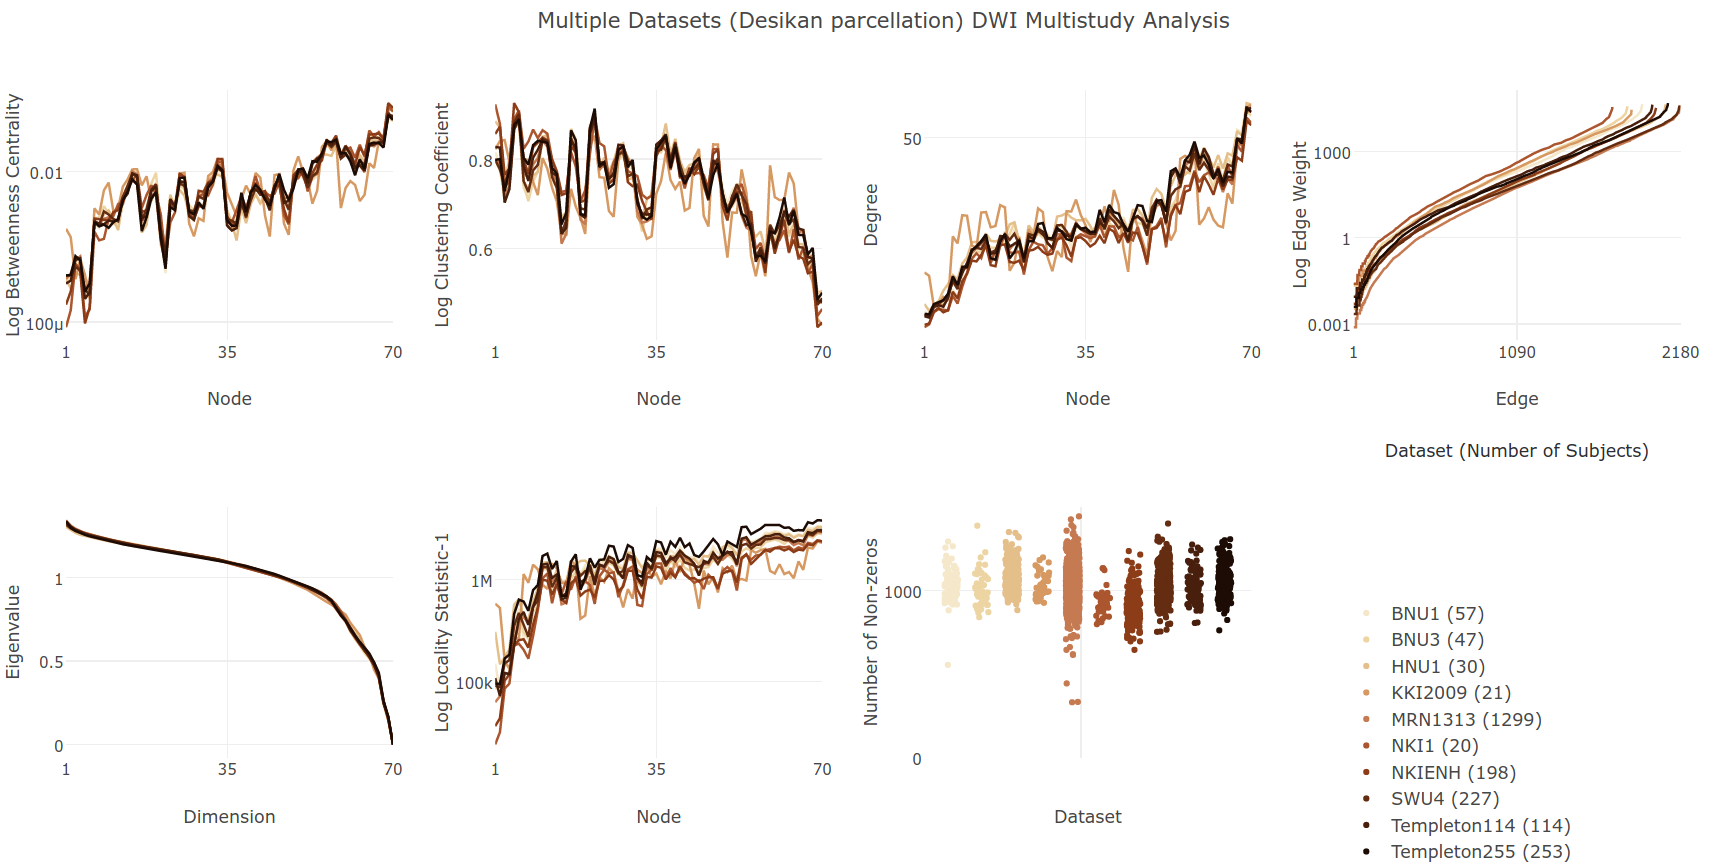
\includegraphics[width=\textwidth]{./figs/fig_dwi_multisite.png}
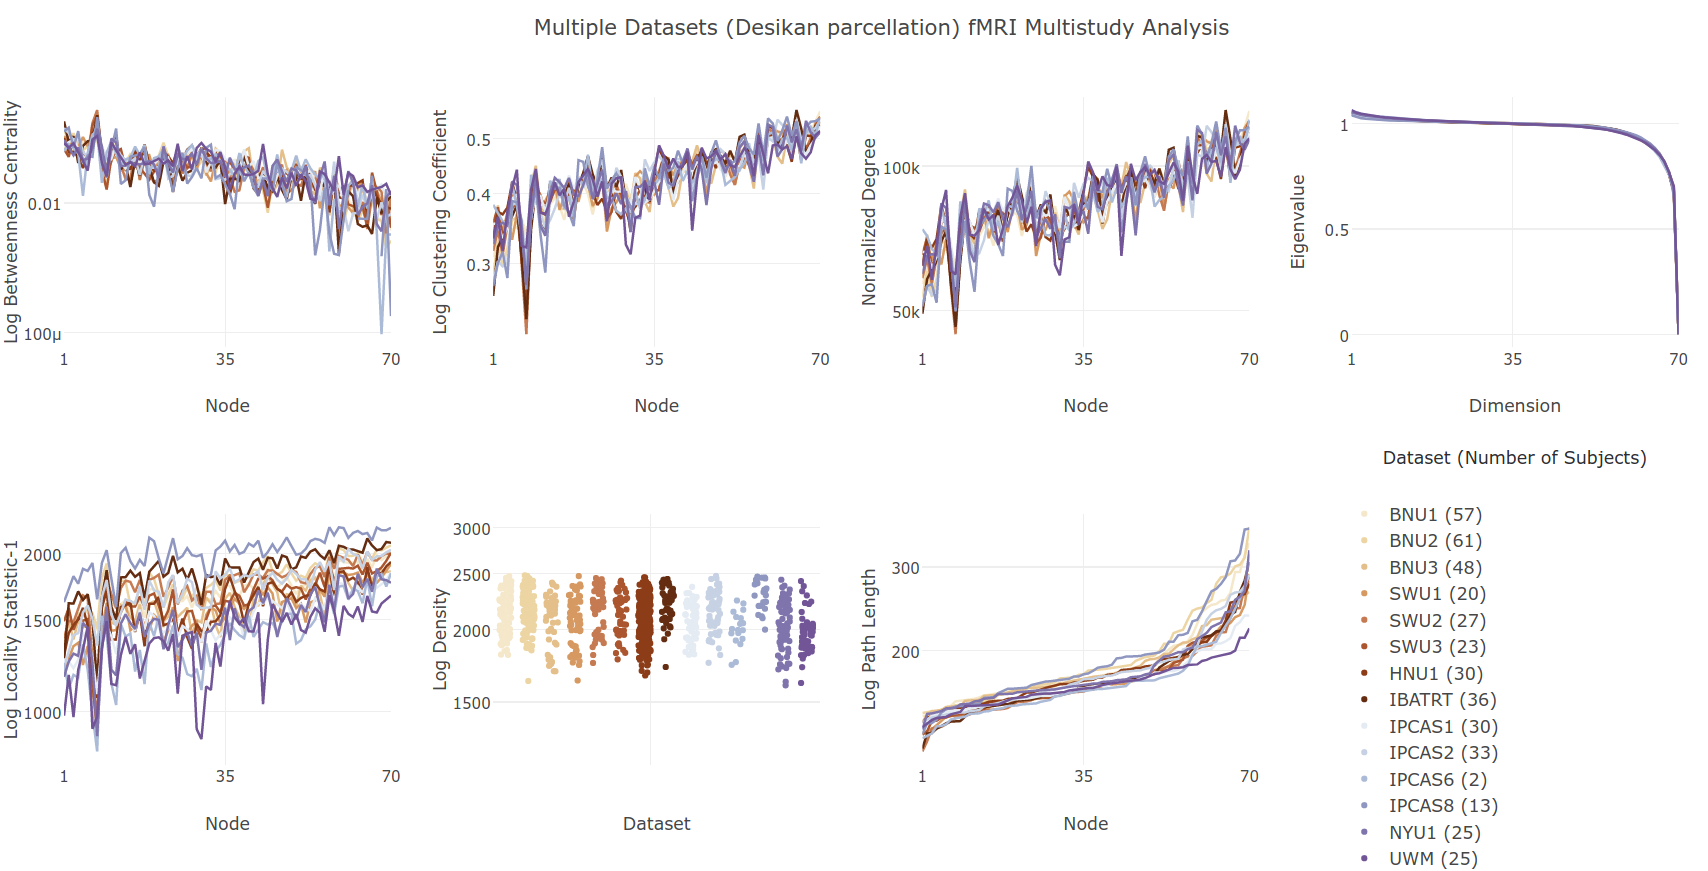
\includegraphics[width=\textwidth]{./figs/fig_fmri_multisite.png}
\caption{
\textbf{Multi-Study Connectome Analysis}.
Average connectomes from ten diffusion studies processed with \ndmgd~are qualitatively compared by way of their summary statistics on the Desikan parcellation in the top figure.
The Desikan atlas used in \ndmg~has been modified to include two additional regions, one per hemisphere, which fills in a hole in the parcellation near the corpus callosum.
The nodes in this plot have been sorted such that the degree sequence of the left hemisphere (Desikan nodes 1-35) of the BNU1 dataset is monotonically non-decreasing, and that corresponding left-right nodes are next to one another.
Each line shows the average for each statistic over all individuals within the study.
On  the bottom, we repeat the same analysis on the functional connectomes from seventeen different studies. Like the statistics computed in for the diffusion connectomes, the statistics are again qualitatively similar but quantitatively disparate. This suggests that claims made or analyses
performed on a given scale may not hold when applied to another scale. Again, we see that parcellation choice has an impact on the implications of a study. Information on the graph statistics computed can be found in \ref{app:graphstats}.}
\label{fig:multisite}
\end{figure*}